%%% Chapter heading commands %%%

%\setlength{\headsep}{15pt}

\renewcommand{\publ}{\flushleft\footnotesize{Published as:\\[0.1cm]
K. Bunte, P. Schneider, B. Hammer, F.-M. Schleif, T. Villmann and M. Biehl -- \textit{``Discriminative Visualization by Limited Rank Matrix Learning,''} Leipzig University, Machine Learning Reports (2:3), %no.\ 3
% , vol. 2, 
pp. 37--51, 2008.\\[0.1cm]
K. Bunte, P. Schneider, B. Hammer, F.-M. Schleif, T. Villmann and M. Biehl -- \textit{``Limited Rank Matrix Learning Discriminative Dimension Reduction and Visualization,''} accepted for publication in Neural Networks 2011.\\}}

\chapter{Limited Rank Matrix LVQ}
\label{chapter:LiRaMLVQ}

\epigraph{Projection makes it possible.}{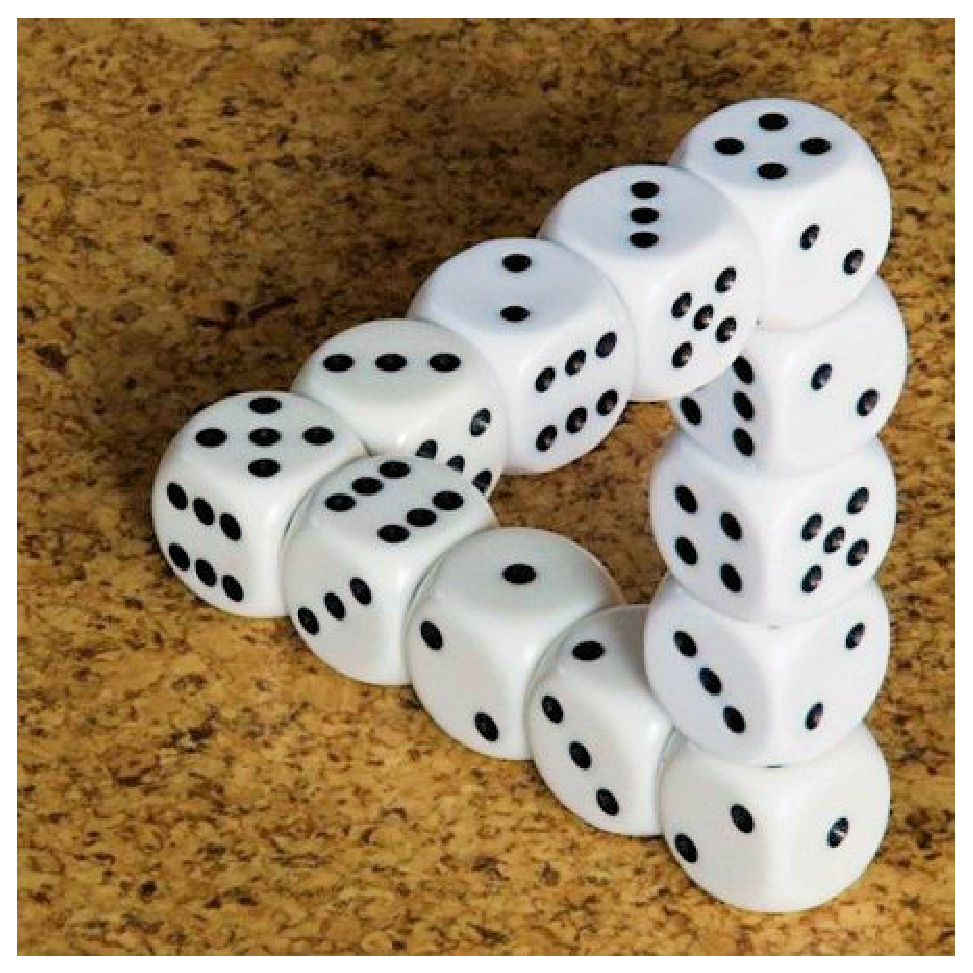
\includegraphics[width=2.5cm]{pics/dice_ShigeoFukuda.eps}\\The impossible triangle. Shigeo Fukuda}

\index{Adaptive Metrics}

%%% Abstract %%%

\begin{Abstract}
We present an extension of the %recently introduced 
Generalized Matrix Learning Vector Quantization algorithm. 
In the original scheme, adaptive square matrices of relevance factors parameterize a discriminative distance measure. 
We extend the scheme to matrices of limited rank corresponding to low-dimensional representations of the data. 
This allows to incorporate prior knowledge of the intrinsic dimension and to reduce the number of adaptive parameters efficiently. 
In particular, for very high dimensional data, the limitation of the rank can reduce computation time 
and memory requirements significantly. 
Furthermore, two- or three-dimensional representations constitute an efficient visualization method for labeled data sets. 
The identification of a suitable projection is not treated as a pre-processing step but as an integral part of the supervised training.  
Several real world data sets serve as illustration and demonstrate the usefulness of the suggested method.
\end{Abstract}

%%% Chapter sections %%%
% \index{Visual system}
% \iffalse
\section{Introduction}

\PARstart{I}n~\cite{Schneider2009a,Schneider2009b} the concept of \ac{GMLVQ} is introduced. 
% An important extension of this concept has been introduced in 
% in  the so-called Generalized Matrix LVQ (GMLVQ) a 
It uses the quadratic form Eq.\ (\ref{eq:d_Lambda}) as distance including a full matrix of relevances, 
which can account for correlations between different features. 
An adaptive self-affine transformation $\Omega$ (see Eq.\ (\ref{eq:Lambda})) of feature space identifies the coordinate 
system which is most suitable for the given classification task. 
The original formulation of \ac{GMLVQ} employs symmetric squared  matrices $\Omega\in\R^{N\times N}$ and 
is summarized in Algorithm \ref{alg:GMLVQ}. 
In the simplest case, one matrix is taken to define a global distance measure. 
Extensions to class-wise or local matrices, attached to individual prototypes Eq.\ (\ref{eq:d_Lambda_j}), 
are technically straightforward and allow for the parameterization of more complex decision boundaries. 

In this chapter we present and discuss an important modification: the use of rectangular transformation 
matrices $\Omega\in\R^{M\times N}$ with $M\le N$ \cite{MLR0308Bunte2008a,Bunte2011_LiRaMLVQ}%\cite{MLR0308Bunte2008a,Bunte_LiRaM_LVQ_2011}
.\newnot{symbol:M} 
The corresponding relevance matrices $\Lambda$ are of bounded rank $M$ or, in other words, distances are 
evaluated in a space with reduced dimension, see Eq.\ (\ref{eq:transformation}). 
The motivation for considering this variation of \ac{GMLVQ} is at least two-fold: 
% \begin{itemize}
% \item[(a)] 
(a) prior knowledge about the intrinsic dimension of the data can be incorporated efficiently and 
% \item[(b)] 
(b) the number of free parameters in the learning problem may be reduced significantly. 
% \end{itemize}

Although unrestricted \ac{GMLVQ} displays a tendency to reduce the rank of the relevance matrices in the training process, 
the advantages of restricting the rank explicitly are obvious. 
In particular for nominally very high-dimensional data, e.g.\ in image analysis or bioinformatics, 
unrestricted relevance matrices become intractable. 
In addition, optimization results can be poor when the search is performed in an unnecessarily large parameter space. 
Furthermore, the exact control of the rank allows for pre-defining the dimension of the intrinsic representation and 
is, for instance, suitable for the discriminative visualization of labeled data sets. 
In contrast with many other schemes that consider dimension reduction as a pre-processing step, our method
performs the training of prototypes and the identification of a suitable transformation simultaneously. 
Hence, both sub-tasks are guided by the ultimate goal of implementing the desired classification scheme.  

Appropriate projections into two- or three-dimensional spaces can furthermore be used for efficient visualization of labeled data. 
Visualization enables to use the astonishing cognitive capabilities of humans for visual perception when extracting 
information from large data volumes. 
Structural characteristics can be captured almost instantly by humans, independent of the number of displayed points. 
Classical unsupervised dimension reduction techniques represent data points contained in a
high dimensional data manifold by low dimensional counterparts in, for instance, two
or three dimensions, while preserving as much information as possible. 
Since it is not clear in advance which parts of the data are relevant to the user, this problem is inherently
ill-posed: depending on the specific data domain and the situation at hand, different aspects can be in the focus of attention. 
Prior knowledge, in form of label information, can be used to formulate a well-defined objective in terms of the 
classification performance. 

There exist a few classical dimensionality reduction tools which take class labels into account:
e.g.\ Classical Fisher \ac{LDA}, the recently introduced \ac{LFDA} \cite{Sugiyama2007}, 
\ac{NCA} \cite{Goldberger2004}, as well as \ac{PLS}. %offer supervised linear visualization techniques. 
\index{Dimension Reduction!Supervised methods!LDA}
\index{Dimension Reduction!Supervised methods!LFDA}
\index{Dimension Reduction!Supervised methods!PLS}
\index{Dimension Reduction!Supervised methods!NCA}
These methods can be extended to nonlinear projections by kernel methods \cite{Ma2007,Baudat2000}.  
% Kernel methods extend these settings to nonlinear projections \cite{Ma2007,Baudat2000}.
Adaptive dissimilarity measures which modify the metric %used for projection 
according to the given auxiliary information have been introduced e.g.\ in 
\cite{Kaski2001,Peltonen2004,Bunte_ESANN2009a,Bunte_CAIP2009_NLdimred,BunteESANNSI2009}.%,BunteESANNSI2009,
The resulting metric can be integrated into various techniques such as \ac{SOM}, \ac{MDS}, 
\index{Dimension Reduction!Unsupervised methods!SOM}
\index{Dimension Reduction!Unsupervised methods!MDS}or a recent information theoretic
model for data visualization \cite{Kaski2001,Peltonen2004,Venna2010}.
An ad hoc metric adaptation is used in \cite{Geng2005} to extend Isomap \cite{Tenenbaum2000} to class labels.
Alternative approaches change the cost function of dimensionality reduction, for instance 
by using conditional probabilities, class-wise similarity matrices 
or introducing a covariance-based coloring matrix for the side information as proposed in \cite{Iwata2007,Memisevic2005,Song2008}. 
The detailed explanation of the most important supervised and unsupervised dimension reduction techniques is 
given in Part \ref{part:2} %``Dimension Reduction and Visualization'' 
of this thesis. 

In the next section we describe the \ac{LiRaM LVQ} as extension of the original \ac{GMLVQ} formulation. 
%Sec.\ \ref{section:rectangular} we review GMLVQ in the following section.  
Afterwards we apply the novel approach to a benchmark problem and study the influence of the dimension 
reduction on the classification performance. 
We also compare the limited rank version to the naive approach of taking the first components of the full rank \ac{GMLVQ}. 
We show that reducing the rank after training not only requires more memory and CPU time, 
but also yields inferior classification performance compared to \ac{LiRaM LVQ}. 
In Sec.\ \ref{sec:LiRaM_LVQ_visualization} we present example applications of our algorithm in the visualization of labeled data. 
We also compare with visualizations obtained by \ac{LFDA} and \ac{NCA}. 
We conclude by summarizing our findings and providing an outlook on perspective investigations.